\documentclass{article}

% Encoding and fonts to handle Unicode and improve typesetting
\usepackage[utf8]{inputenc}
\usepackage[T1]{fontenc}
\usepackage{lmodern}
\usepackage{microtype}

% NeurIPS style (ensure the .sty file is available in the project)
\usepackage[preprint]{neurips_2023}  % or [final] for camera-ready, [nonatbib] if not using natbib

% Optional packages (already loaded or permitted by NeurIPS guidelines)
\usepackage{graphicx}
\usepackage{booktabs}
\usepackage{amsmath,amssymb}
\usepackage{natbib}
\usepackage{hyperref}
\usepackage{url}
\bibliographystyle{plainnat}

% TikZ for figures
\usepackage{tikz}
\usetikzlibrary{arrows.meta,positioning,shapes.geometric}

% Custom commands (if any)
\newcommand{\PAL}{\textsc{PAL}}  % e.g., acronym for Public Announcement Logic
\newcommand{\CoT}{CoT}          % Chain-of-Thought shorthand

\title{Verifiable Epistemic Alignment for LLM Agents:\\ Public Announcements, Norms, and Chain-of-Thought Verification}

\author{
    Justin Mullins \\
    University of Kansas \\
    Center for Cyber Social Dynamics \\
    \texttt{jpmullins2621@gmail.com} \\
    \And
    John Symons \\
    University of Kansas \\
    Center for Cyber Social Dynamics \\
    \texttt{email@example.com}\\
}

\begin{document}

\maketitle

% Abstract
\begin{abstract}
Recent advances in large language model (LLM) agents have highlighted the need for epistemic alignment: the agent's internal beliefs and reasoning steps must remain consistent with reality and with human-provided norms. We propose a framework to achieve verifiable epistemic alignment by integrating a formal epistemic state layer and a verification gate into the LLM's decision loop. The epistemic state layer tracks the agent's knowledge as logical propositions ($\Sigma$), updating this state via public announcement logic (\PAL) whenever the agent acquires new information or deduces new facts. Alignment norms, such as safety or ethical rules, are encoded as logical constraints in the same framework. At each reasoning step, the agent's chain-of-thought (\CoT) is passed through a neuro-symbolic verification gate that checks for logical consistency, valid entailment, and grounding of claims. If a proposed thought contradicts known facts or norms, or introduces unsupported assumptions, the gate flags it for revision. This yields a self-correcting reasoning process where the LLM's intermediate conclusions must be \emph{proved} or \emph{justified} with respect to its knowledge base and norms. We present the architecture and formalism of this epistemic alignment mechanism, describe a reference implementation, and evaluate it on reasoning benchmarks and safety-critical tasks. The results indicate that our approach effectively identifies and eliminates reasoning errors, enforces compliance with norms, and improves the interpretability of the agent's decision-making. This work paves the way for LLM agents that can explain, verify, and refine their own reasoning in line with what they know and what they are allowed to do.

\end{abstract}

% Sections
\section{Introduction}
Large language models (LLMs) have rapidly become the core reasoning engines for AI agents. However, their impressive performance is tempered by a lack of reliable internal self-monitoring. They often produce confident multi-step reasoning (via chain-of-thought prompting) that contains logical errors or unfounded assumptions, even if the final answer appears correct. In high-stakes domains like law or medicine, it is not enough for an agent to get the right answer, the validity of its reasoning process and adherence to human norms are equally critical. Recent work has introduced the notion of an LLM's epistemic agency, the ability to form, update, and monitor its beliefs about the world. Reliability and trustworthiness of AI agents “critically hinge on their intrinsic epistemic agency,” yet current LLMs show only rudimentary signs of this capacity. We address this gap by proposing a framework for verifiable epistemic alignment, which ensures that an LLM agent's intermediate reasoning remains logically sound and aligned with explicit knowledge and norms at every step.

Our approach introduces two key ideas: (1) an epistemic state layer that explicitly tracks what the agent knows or assumes, and (2) a verification mechanism that checks each chain-of-thought (CoT) step against that state for truthfulness, consistency, and norm compliance. The epistemic state is represented in a formal logic where adding a new piece of information is akin to making a public announcement to oneself, eliminating possibilities incompatible with that information. This lets the agent update its knowledge rigorously whenever it observes new evidence or deduces a fact. Norms, e.g., safety rules or ethical principles, are encoded in the same logical form, so they act as inviolable axioms in the knowledge base. The verification mechanism is a neuro-symbolic verification gate interposed in the agent's reasoning loop. Before accepting any self-generated thought or taking an action, the agent uses a logical solver to verify that the proposal:
\begin{itemize}
\item does not contradict the current knowledge base (including norms);
\item is logically entailed or supported by known premises (or explicitly marked as an assumption); and
\item is grounded in provided information (not an unexplained leap or hallucination).
\end{itemize}

If a step fails these checks, the agent is prompted to reconsider or explain the step, enabling a form of self-correction (in spirit similar to reflective LLM approaches) but with formal logic criteria. Through this loop, the LLM agent effectively verifies its own reasoning as it proceeds, rather than relying solely on post-hoc critique.

\subsection{Motivation and Contribution}
The motivation for our framework arises from limitations in current LLM agent strategies. Standard chain-of-thought prompting improves reasoning outcomes but offers no guarantee of internal validity, an LLM may introduce a false intermediate claim that goes unchallenged. Likewise, alignment techniques like reinforcement learning from human feedback target final outputs but do not enforce consistency of the reasoning process. Our work bridges formal epistemic logic with LLM reasoning to fill this gap. Specifically, we contribute:
\begin{enumerate}
\item \textbf{Epistemic alignment layer}: a novel architecture that augments an LLM agent with an explicit epistemic state (knowledge base) and an update rule based on Public Announcement Logic (PAL). This ensures new information is integrated transparently and is logically analyzable.
\item \textbf{Norm encoding in logic}: a method to translate natural language norms or instructions into formal constraints that the agent's reasoning must obey. We demonstrate how high-level directives (e.g., “the agent should not reveal private data”) can be formalized and checked within the reasoning loop.
\item \textbf{Chain-of-thought verification gate}: a neuro-symbolic verification mechanism that intercepts the LLM's intermediate reasoning steps. We formalize the verification criteria (no contradictions, valid inference, sufficient grounding) and implement it using an automated theorem prover, yielding a system that can catch reasoning errors or hallucinations in real time (e.g., extending the spirit of \citet{feng2025vericot}).
\item \textbf{Evaluation on reasoning and safety tasks}:
  \begin{enumerate}
  \item Logical reasoning benchmarks (e.g., ProofWriter) where complex multi-step deduction is required.
  \item Safety-oriented tasks (e.g., Reflection-style and adversarial user queries).
  \end{enumerate}
  We show that the epistemic alignment layer improves logical consistency and reduces norm violations, with ablation studies confirming the contribution of each component.
\end{enumerate}

\section{Background}
Our approach intersects two domains: formal epistemic logic (for representing knowledge, belief, and informational changes) and LLM chain-of-thought reasoning (for generating and evaluating reasoning steps in natural language). We briefly review key concepts from each domain and related prior work that informs our solution.

\subsection{Epistemic Logic and Public Announcements}
Epistemic logic is the logic of knowledge and belief. In the classical epistemic logic (often modeled as modal logic S5), an expression $K_i \varphi$ means “agent $i$ knows $\varphi$.” Semantically, this is evaluated on a set of possible worlds with an accessibility relation for each agent $i$ that relates worlds indistinguishable to $i$. The knowledge operator $K_i$ is typically assumed to be factive ($K_i \varphi \to \varphi$, meaning if $i$ knows $\varphi$, then $\varphi$ is true) and to satisfy positive and negative introspection (agents know what they know and know that they know it, in idealized models). These correspond to axioms $T: K_i\varphi \rightarrow \varphi$, $4: K_i\varphi \rightarrow K_iK_i\varphi$, and $5: \neg K_i\varphi \rightarrow K_i(\neg K_i\varphi)$ in modal logic, characterizing the S5 system.

A key extension is Dynamic Epistemic Logic (DEL), which studies how knowledge changes as a result of events or observations. One of the simplest and most well-studied DEL frameworks is Public Announcement Logic (\PAL). In \PAL, an announcement of a formula $\psi$ (usually written $[\psi]!$) is an action that eliminates all possible worlds where $\psi$ is false, effectively updating every agent's knowledge to $\psi$. After a truthful public announcement, all agents come to know $\psi$ (assuming they heard it). For example, if it is publicly announced that “$p$ is true,” then in the updated model $K_i p$ holds for all agents $i$. In our context, we use \PAL as an analogy: when our single LLM agent uncovers a new fact or receives new information, we treat it as a (virtual) public announcement to itself, updating its epistemic state $\Sigma$. By doing so, we ensure the agent's knowledge base is always an update of prior knowledge with new truths.

Beyond classical binary logic, researchers have explored non-classical and graded epistemic logics to handle uncertainty or partial belief. \citet{li2022graded} introduce a graded many-valued modal logic with rough truth. While our current work doesn't explicitly use graded truth values, the concept is relevant for future extensions: an LLM could associate confidence levels with beliefs, and a graded epistemic logic could model statements like “the agent is 90\% sure of $\varphi$.” For now, we assume a bivalent logic (each proposition is either accepted or not in the agent's knowledge base), but acknowledge that extending to graded beliefs is an interesting avenue.

Another extension relevant to norms is deontic logic (logic of obligations and permissions). Although we do not explicitly delve into deontic modalities, encoding norms as logical constraints in $\Sigma$ can be seen as adding formulas that must always be true (akin to obligations that the agent should consider as inviolable). This parallels the idea of treating certain propositions as axioms that announcements cannot contradict.

\subsection{Epistemic Planning and Knowledge in AI Agents}
Epistemic logic has been used in AI planning to represent and reason about the knowledge states of agents. For example, epistemic planning problems involve actions that have not only physical effects but also informational (knowledge-altering) effects. A classic challenge is representing how an agent's knowledge changes when it performs sensing actions or communicates with others. \citet{occhipinti2020dynamic} extend DEL with first-order quantification, enabling more expressive representations of multi-agent knowledge and actions (like “agent $a$ knows that some block is red”). They introduce term-modal logics where modal operators can be indexed by terms (agents or objects) to compactly model scenarios with many agents or objects. These sophisticated formalisms highlight that keeping track of “who knows what” can become complex, but also that logic provides tools to do so systematically.

In our single-agent setting, the planning problem simplifies (we track only the LLM's knowledge). However, inspirations can be drawn from epistemic planning: for instance, the notion of an action model that specifies preconditions and effects on knowledge. One could imagine each tool invocation or environment interaction by the agent as an action with an associated epistemic effect (“after querying the database, the agent knows the returned fact”). We do not explicitly construct action models here, but our framework can be viewed as an epistemic planning loop where the agent's actions include both world-interactions and introspective actions (like checking for consistency, which update the agent's meta-knowledge about its beliefs).

Knowledge graphs and memory: Outside of formal logic, LLM-based agents such as Generative Agents by \citet{park2023generative} have implemented long-term memory by storing past events and facts in natural language and retrieving them when needed. Our approach can be seen as creating a structured memory (the logical state $\Sigma$) which is analogous to a knowledge graph or database of facts the agent believes. The difference is that our memory is principled: it is maintained through logical rules (public announcement updates) rather than heuristic summarization, and it supports inference via the verification gate. This principled approach trades some flexibility for guarantees of consistency. Notably, Park et al. found that certain implicit norms (like “bathrooms can only have one occupant”) did not emerge in their generative agents unless explicitly encoded. This aligns with our motivation to encode norms explicitly: an agent's memory or world state should include not just factual observations but also contextual rules so that it does not violate common-sense or domain-specific constraints.

\subsection{Chain-of-Thought Reasoning in LLMs and Verification}
Chain-of-Thought (CoT) prompting is a technique where an LLM is prompted to generate a step-by-step reasoning trajectory before giving a final answer. Empirically, CoT has improved performance on math, commonsense, and multi-hop reasoning tasks by allowing the model to decompose complex queries. However, CoT by itself does not guarantee correctness of each step. An LLM might produce a convincing rationale that contains a logical leap or hallucinated fact. Because the final answer can still be correct by coincidence or because errors cancel out, purely outcome-based evaluation would miss these flaws. This is problematic especially if users or downstream systems rely on the reasoning (for interpretability or justification).

Researchers have begun exploring self-verification and reflection for CoT. One line of work is using a separate critic model or an iterative refinement loop where the LLM assesses and improves its own output. For example, \citet{shinn2023reflexion} proposed the Reflexion framework where after an initial attempt, the agent uses feedback (e.g., failed tests or error signals) to reflect and adjust its actions, storing lessons in a dynamic memory. This improved success on coding tasks and interactive games without additional training, by allowing the model to learn from mistakes. Reflexion, however, relies on heuristic feedback (e.g., an error message from a code compiler, or the agent noticing it is repeating actions) rather than a formal logic check. Our approach can be seen as providing a logical feedback signal for reflection: the verification gate supplies explicit reasons (contradiction, ungrounded inference) why a thought is unacceptable, which the LLM can then use to guide its self-correction.

Another relevant work is VeriCoT by \citet{feng2025vericot}, which introduced a neuro-symbolic method to check the internal logic of chain-of-thought. VeriCoT automatically translates each step of an LLM's reasoning into formulas in first-order logic and identifies the supporting premises (from the context or prior steps) for that step. With this formal trace, they use automated theorem provers to verify if each step is logically valid. They demonstrated on tasks like ProofWriter and legal reasoning that VeriCoT can effectively flag flawed reasoning and that a verification score correlates with whether the final answer is correct. We draw significant inspiration from VeriCoT's approach to ground and check CoT steps. The key difference is that we integrate the verification into the agent's generation loop. Whereas VeriCoT operates as an analysis after a chain is produced (or as a training signal to fine-tune models), we place a “live” verification step between each thought to immediately catch errors. This real-time checking required us to adapt the paradigm: the agent knows it will be checked, and can adjust its strategy (for example, being more explicit about justifications). In essence, our work extends VeriCoT by making verification part of the agent's deliberation, not just an external evaluator.

Finally, our work relates to the broader notion of truthful AI and safe AI. Efforts such as Constitutional AI (Anthropic, 2023) and OpenAI's system coaching involve an LLM following a set of written principles to critique and refine its outputs. Our norm-encoding can be seen as a formal counterpart: instead of (or alongside) heuristic prompt-based critiques (“Assistant should avoid content X”), we enforce certain principles through logic. This provides a clear criterion for violation (a norm formula becomes false, causing inconsistency). It also has the benefit of being transparent: one can inspect the norm formulas in $\Sigma$ to see exactly what rules the agent is following. Recent benchmarks like Reflection-Bench include tasks for belief updating and meta-reflection; our architecture is naturally suited to such tasks because it builds belief updates and reflection (via verification) into the agent's core loop.

In summary, the background threads we build upon are: the formal tools for representing knowledge and its dynamics (from epistemic logic), and the emerging techniques for aligning and verifying LLM reasoning (from CoT prompting, reflexion, and neuro-symbolic validation). The convergence of these threads leads to our proposed solution, which we now detail.

\section{Epistemic Alignment Architecture}\label{sec:architecture}
At the heart of our approach is an Epistemic Alignment Layer that wraps around a standard LLM agent. This layer endows the agent with an explicit, manipulable representation of its knowledge and a process to verify reasoning steps. Figure~\ref{fig:loop} gives a high-level overview of the agent's decision loop with this layer in place, which we summarize first:

\begin{figure}[t]
  \centering
  \begin{tikzpicture}[node distance=3cm, >=Stealth,
    process/.style={draw, thick, rounded corners, align=center, fill=blue!20, minimum width=2.5cm, minimum height=1cm},
    state/.style={draw, thick, ellipse, align=center, fill=gray!20, minimum width=1.2cm, minimum height=0.8cm}]
    % Nodes (epistemic loop stages)
    \node[process] (observe) {Observe};
    \node[process, right=of observe] (parse) {Parse};
    \node[process, right=of parse] (verify) {Verify};
    \node[process, right=of verify] (update) {Update (PAL)};
    \node[process, right=of update] (reason) {Reason};
    \node[process, right=of reason] (act) {Act};
    \node[process, right=of act] (feedback) {Feedback};
    % Knowledge state Sigma
    \node[state, above=1.2cm of update, xshift=-1cm] (sigma) {$\Sigma$};
    % Main loop arrows
    \draw[->, thick] (observe) -- (parse);
    \draw[->, thick] (parse) -- (verify);
    \draw[->, thick] (verify) -- (update);
    \draw[->, thick] (update) -- (reason);
    \draw[->, thick] (reason) -- (act);
    \draw[->, thick] (act) -- (feedback);
    % Feedback loop (arrow from Feedback back to Observe)
    \draw[->, thick] (feedback.south) .. controls ($(feedback.south)+(0,-2)$) and ($(observe.south)+(0,-2)$) .. (observe.south);
    % Verification gate connections with state Sigma
    \draw[->, thick, dashed] (sigma.south) -- (verify.north);
    \draw[->, thick, dashed] (update.north) -- (sigma.south);
\end{tikzpicture}

  \caption{Reasoning loop for the epistemically aligned agent. The agent observes new input, verifies candidate chain-of-thought (CoT) steps against its current knowledge and norms, updates the epistemic state $\Sigma$ with approved information (modeled as a public announcement), and then acts.}
  \label{fig:loop}
\end{figure}

Crucially, the verification step can trigger a revision: if the CoT step is not verified, the agent will rethink or adjust the step before updating $\Sigma$ or taking an external action. We now describe each component of the architecture in detail:

\subsection{Epistemic State $\Sigma$ and Knowledge Initialization}
We denote the agent's epistemic state as $\Sigma$ (sigma), which is a set of logical formulas representing everything the agent currently knows or takes to be true. Initially, $\Sigma$ is constructed from the task prompt and any prior context. For example, if the user asks a question with some background, those facts are included in $\Sigma$. Domain assumptions or common knowledge can also be seeded here (though one must be careful, if the agent is allowed to assume all of human common sense, $\Sigma$ could be very large. In practice we include only key facts or explicitly provided knowledge, and rely on the LLM's latent knowledge for trivial commonsense, checking as needed).

Formally, $\Sigma$ might be represented in a suitable logical language. A convenient choice is first-order logic (FOL) for expressiveness. Each atomic fact from the environment (e.g., "Alice is Bob's mother") can be a predicate $Mother(Alice, Bob)$ in $\Sigma$. Norms can be represented as universally quantified implications (e.g., "for any person $x$, do not reveal $x$'s home address" could be a formula $\forall x\, \neg \textit{RevealAddress}(x)$ in $\Sigma$. In implementation, we might use a logical knowledge base or a semantic graph; the specific representation can vary as long as it supports entailment checks.

Before the agent begins reasoning on a new problem, $\Sigma$ is initialized with:
\begin{itemize}
\item Environment facts: Any information provided by the user or environment (e.g., a context paragraph for a QA task, or the current state of a game world).
\item Persistent agent knowledge: This could include previously learned facts (for a long-lived agent across sessions) or domain knowledge. In a stateless question-answering scenario, this may be empty or minimal.
\item Norms and constraints: A set of logical formulas encoding what the agent should or should not do. These act like axioms, they are intended to remain true throughout and the agent should never knowingly violate them.
\end{itemize}

By treating norms as part of $\Sigma$, we ensure any potential violation would appear as an inconsistency (contradiction) when combined with a violating action. For instance, if $\Sigma$ contains $\forall x\, \neg \textit{RevealAddress}(x)$ and the agent's thought is "I will reveal Alice's address," that thought can be translated to $\textit{RevealAddress}(Alice)$ which clearly conflicts with the axiom (making $\Sigma \cup \{\textit{RevealAddress}(Alice)\}$ unsatisfiable). This mechanism will be caught by the verification gate (Section~\ref{sec:verification}).

\subsection{Public Announcement Updates in Reasoning}
As the agent reasons, it generates intermediate conclusions or sub-answers. In our framework, each time the agent is about to accept a new piece of information as true, we model it as a PAL-style update: $\Sigma := \Sigma \land \varphi$, where $\varphi$ is the new formula (announcement). This is conceptually the same as the public announcement $[\varphi]!$ in dynamic epistemic logic, except here there is only one agent (the LLM itself) and we assume $\varphi$ is true in the actual world (the agent believes it as truth). The effect is to restrict $\Sigma$ to worlds where $\varphi$ holds, effectively adding $\varphi$ to the knowledge base.

For example, suppose the agent has $\Sigma$ containing "If A is B's parent, then A is older than B," and during reasoning it deduces "Alice is older than Bob." Before adding this as knowledge, the agent should verify it. Assuming it checks out (Alice is Bob's mother was known, so by the rule, yes Alice is older), the agent performs a public announcement update with $\varphi = Older(Alice, Bob)$. Any subsequent reasoning will then include $Older(Alice, Bob)$ as a known fact. If, later in the dialogue, the user provides new information that Bob is actually older than Alice, adding that would conflict with $Older(Alice, Bob)$ already in $\Sigma$; our system would catch this conflict and could either reject the new info or flag the inconsistency (depending on design, see Section~\ref{sec:discussion} on limitations).

It is important to note that not every step of the LLM's chain-of-thought should necessarily become a public announcement. Sometimes the model might consider a hypothetical or an uncertain guess. We allow the agent to distinguish between tentative assumptions and solid conclusions:
\begin{itemize}
\item Tentative assumption: can be phrased as such and not immediately added to $\Sigma$ as truth. We might handle this by introducing it with a special marker (e.g., "Suppose $\varphi$ for sake of argument..."). The verification gate can then treat it differently, perhaps checking consistency of the assumption but not requiring it to be entailed by $\Sigma$.
\item Solid conclusion: if the agent is confident it is true, it would be added to $\Sigma$.
\end{itemize}

In practice, to keep things simple, our implementation currently treats each CoT step that the model asserts as a fact as an addition to $\Sigma$ (after verification). If the model wishes to consider a hypothesis, we expect it to explicitly say so (and we could model that with a different operation, like a tagged formula in $\Sigma$ or a branch in reasoning). Managing multiple possible worlds or branches is beyond the scope of this work, but Section~\ref{sec:discussion} touches on this as a future direction (related to non-monotonic reasoning and exploring what-if scenarios).

\subsection{LLM-as-Judge and Norm Adherence}
While a logical solver provides the backbone for verification, we incorporate the LLM itself as a judge in two ways:
\begin{enumerate}
\item Norm interpretation: Norms provided in natural language (e.g., a policy document or user instructions like "avoid hateful language") may require interpretation. We utilize the LLM to translate such NL descriptions into formal constraints. For instance, the prompt to the LLM-as-judge might be: "Translate the following guideline into a logical condition the agent must satisfy: 'The assistant should not reveal personal identifiable information (PII).'" The LLM might respond with something like a logical template $\neg \textit{Reveal}(x)$ if $x$ is PII. A developer or a higher-level system could confirm and refine this formalization. The resulting formula(s) go into $\Sigma$. Essentially, the LLM helps bootstrap the formal knowledge of norms.
\item Contextual judgment: Some situations are too fuzzy for hard logic. For example, determining if a certain statement constitutes "hateful language" might be non-trivial to formalize with simple logical rules, it might require semantic understanding and context. In such cases, we can ask the LLM-as-judge (potentially a separate instance or prompt of the model) to evaluate whether a candidate output violates the spirit of a norm. This is akin to a natural language inference or classification task for the model. If the LLM-as-judge says "Yes, this seems violative because ...," we can treat that as a signal to reject or modify the output.
\end{enumerate}

We emphasize that the LLM-as-judge is used when formal logic alone does not suffice. Whenever a norm can be concretely encoded (like "never output a 5-digit number as it might be a zip code", a contrived example), a direct logical constraint is preferred because it is unambiguous and checkable by the solver. The LLM judge is a fallback for nuanced content evaluation.

Figure~\ref{fig:charity} illustrates a "norm pipeline," using an example scenario where the agent has a norm about charitable behavior.

\begin{figure}[t]
  \centering
  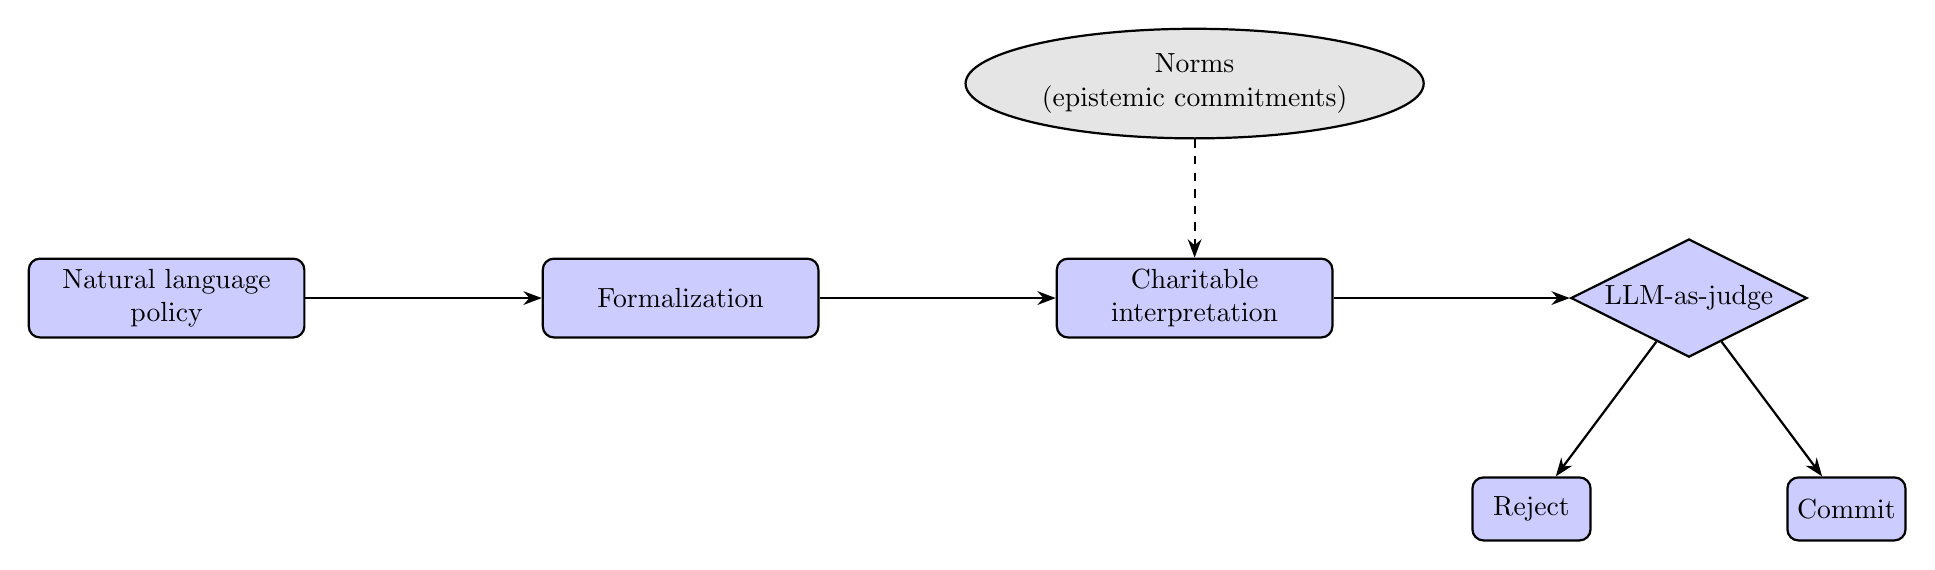
\begin{tikzpicture}[>=Stealth,
    process/.style={draw, thick, rounded corners, align=center, fill=blue!20, minimum width=3.5cm, minimum height=1cm},
    decision/.style={draw, thick, fill=blue!20, diamond, aspect=2, inner sep=1pt, minimum width=3cm, minimum height=1.5cm, align=center},
    outcome/.style={draw, thick, rounded corners, align=center, fill=blue!20, minimum width=1.5cm, minimum height=0.8cm},
    state/.style={draw, thick, ellipse, align=center, fill=gray!20, minimum width=3.5cm, minimum height=0.8cm}]
    % Nodes (normative pipeline stages)
    \node[process] (nlpolicy) {Natural language\\policy};
    \node[process, right=3cm of nlpolicy] (formal) {Formalization};
    \node[process, right=3cm of formal] (charity) {Charitable\\interpretation};
    \node[decision, right=3cm of charity] (judge) {LLM-as-judge};
    % Outcome nodes for decision
    \node[outcome, below=1.5cm of judge, xshift=-2cm] (reject) {Reject};
    \node[outcome, below=1.5cm of judge, xshift=2cm] (commit) {Commit};
    % Norms input as epistemic commitments
    \node[state, above=1.5cm of charity] (norms) {Norms\\(epistemic commitments)};
    % Arrows
    \draw[->, thick] (nlpolicy) -- (formal);
    \draw[->, thick] (formal) -- (charity);
    \draw[->, thick] (charity) -- (judge);
    \draw[->, thick] (judge) -- (commit);
    \draw[->, thick] (judge) -- (reject);
    \draw[->, thick, dashed] (norms.south) -- (charity.north);
\end{tikzpicture}

  \caption{Norm interpretation pipeline. Natural-language policies are formalized, interpreted charitably, and reviewed by the LLM-as-judge before new norm commitments are added to $\Sigma$.}
  \label{fig:charity}
\end{figure}

The LLM-as-judge concept is implemented as a special prompting of the same base model (or a smaller model) that is kept separate from the main reasoning chain. It has access to the norm descriptions and possibly the dialogue or state context, but it is prompted to output only a judgment (and rationale if needed). This is similar to a constitutional AI "critique" stage, but here it is integrated with our logical layer. The final arbiter on many checks is still the symbolic solver, e.g., the solver will catch a direct logical contradiction or norm violation. The LLM judge helps where human value judgments are involved.

\subsection{Verification Loop Integration}
With $\Sigma$ and the LLM-as-judge in place, the agent's control flow can be summarized as:
\begin{enumerate}
\item Observation: Get input or perceive environment. Incorporate new facts into $\Sigma$ (after trivial verification if needed). For user-provided info, we generally trust it unless it directly conflicts with $\Sigma$ (handling of conflicting inputs can follow a policy: e.g., user input might override prior knowledge, or the agent might ask for clarification).
\item Proposal: The LLM generates the next step of chain-of-thought (CoT). This could be a sub-answer, an action, or an intermediate deduction.
\item Verification (logic): The proposition(s) in the CoT step are extracted and sent to the verification gate. Here the solver checks consistency: $\Sigma \land \varphi$ (where $\varphi$ represents all new assertions in the step) is tested for satisfiability, and optionally $\Sigma \models \varphi$ is tested for entailment (to judge groundedness).
\item Verification (norms): In parallel, or as part of the consistency check, any formula in $\varphi$ that corresponds to a potential action is checked against norm constraints. If the norms are in $\Sigma$, this is inherently a consistency check. If using the LLM-as-judge for nuance, we call it here.
\item Outcomes:
  \begin{itemize}
  \item If pass (no issues): the step is approved. We update $\Sigma := \Sigma \land \varphi$ (public announcement update) and allow the CoT to continue.
  \item If contradiction: the solver finds $\Sigma \land \varphi$ unsatisfiable, meaning $\varphi$ directly conflicts with something known or an active norm. The agent must revise or abandon $\varphi$. We prompt the LLM (possibly with feedback) to rethink the step. For example: "The last step, '$\varphi$', contradicts what is known or allowed. Please reconsider." The CoT is thereby adjusted (the agent might retract that step or change it).
  \item If ungrounded: $\Sigma \land \varphi$ is consistent but $\Sigma \not\models \varphi$ (i.e., $\varphi$ was not entailed and thus appears to be an assumption or leap). Here the agent is allowed some flexibility. We might either: (a) ask the agent to provide justification ("Explain how $\varphi$ can be derived or provide evidence"), or (b) mark $\varphi$ as an assumption. Depending on context, the agent could continue with $\varphi$ as a new assumption in $\Sigma$ but with a flag that it is unverified. In critical applications, we lean towards option (a), requiring the agent to justify $\varphi$ using known facts (which effectively turns the situation into either entailed or contradicted eventually). Ungrounded steps are where an LLM might hallucinate a fact; catching them prompts the agent either to cite a source or to realize it does not actually know that. This loop resembles the self-reflection proposed by \citet{madaan2023selfrefine} and others, but here triggered by a formal check rather than a heuristic.
  \end{itemize}
\item Action/Output: Once the chain-of-thought yields a final answer or action that is verified, the agent executes that action or outputs the answer. If it is a continuous task, the loop then awaits the next observation and repeats.
\end{enumerate}

This architecture effectively creates a closed-loop system where the LLM's creative generative ability is checked by an unyielding logical standard at each step. The design ensures the LLM is not overly constrained in how it reasons (it can still generate hypotheses, perform reasoning steps in natural language, etc.), but it is constrained in what it can commit to as true or act upon. Only thoughts that pass the epistemic alignment criteria make it into the agent's knowledge state or are used for actions.

The overhead of this process is the extra computation for verification and the possibility of multiple iterations if the LLM initially proposes a flawed step. Our implementation experiences, discussed next, show that with careful engineering, the cost can be kept reasonable and the benefits (averting incorrect or unsafe reasoning) are significant.

\section{Implementation Details}\label{sec:implementation}
We implemented the epistemic alignment layer in a prototype system using Python, combining an LLM (OpenAI GPT-4 API in our experiments) with a logic backend (the Z3 SMT solver for first-order logic consistency checks, and a Prolog engine for simple rule-based reasoning). Here we describe notable aspects of the implementation, including how we represent the knowledge base, how we interface with the LLM for both generation and judgment, and optimizations for efficiency.

\subsection{Knowledge Base Representation and Operations}
The epistemic state $\Sigma$ is represented as a collection of logical assertions. We chose a subset of first-order logic that balances expressiveness with decidability, essentially, relational logic with functions and equality, but no higher-order quantification (to avoid undecidability issues). Each assertion is stored as either:
\begin{itemize}
\item A ground fact (predicate with concrete entities, e.g. $\texttt{Older(Alice,Bob)}$).
\item A rule (Horn-clause style implication or constraint, e.g. $\texttt{Parent}(x,y) \to \texttt{Older}(x,y)$).
\item A norm (which in implementation is just a rule or fact that encodes a prohibition or requirement, e.g. $\texttt{Forbidden}(a)$ for some action $a$).
\end{itemize}

We developed a simple class \texttt{EpistemicState} with methods:
\begin{itemize}
\item \texttt{assert\_fact(formula)}: add a new formula to $\Sigma$ (after verification).
\item \texttt{retract(formula)}: remove a formula (used rarely, e.g., if an assumption is later proven false or in some debugging cases).
\item \texttt{check\_consistency(candidate\_formulas)}: call the Z3 solver to check if $\Sigma \land \text{(candidate formulas)}$ is satisfiable (detects contradictions).
\item \texttt{check\_entailment(candidate\_formula)}: check if $\Sigma \models \text{candidate}$ by asking if $\Sigma \land \neg \text{(candidate)}$ is unsatisfiable (standard refutation).
\end{itemize}

For named entities and predicates, our implementation maintains a symbol table. In many cases, the LLM's outputs are in natural language, so an intermediate step does autoformalization: we crafted prompts that encourage the LLM to output new information in a structured way that can be easily parsed into logical form. For example, if the LLM concludes "Alice is older than Bob", we have it output a tag like \texttt{ASSERT Older(Alice,Bob)} which our code can parse and feed into \texttt{assert\_fact} after verification. This was inspired by the approach of \citet{feng2025vericot}, who had the model annotate each CoT step with a logical translation. We found that by few-shot prompting, GPT-4 could reliably produce statements like \texttt{ASSERT Predicate(arg1, arg2)} for facts, or \texttt{QUERY X} for questions to the solver, etc. These tokens (\texttt{ASSERT}, \texttt{QUERY}) are artificial, purely to facilitate machine parsing.

\paragraph{Exporting to Prompt:} The function \texttt{export\_prompt()} in our code assembles the LLM's prompt at each iteration. It includes:
\begin{itemize}
\item A summary of relevant facts from $\Sigma$. We cannot list all of $\Sigma$ if it grows large, so we employ a relevance filter: given the current goal or question, we select those formulas from $\Sigma$ that have symbols (predicates or constants) overlapping with the goal or the current step's content. This is akin to pulling a support set for the query. For example, if the agent is currently reasoning about ages of Alice and Bob, we include facts like \texttt{Parent(Alice,Bob)} or \texttt{Older(Alice,Charlie)} but omit unrelated facts about other domains. We also always include norm statements in the prompt (since they are few and high-level).
\item An instruction to the LLM to think step-by-step and to formalize any new claims. Essentially: "You are an agent with certain known facts and rules (listed below). You must ensure your reasoning is logically consistent with these and obey the given norms. When you deduce a new fact, state it with an \texttt{ASSERT} tag. If you reach a conclusion or answer, use \texttt{ANSWER} tag. If you find a contradiction or need to check something, you may use \texttt{QUERY}." 
\end{itemize}

The \texttt{QUERY} functionality was added to allow the LLM to explicitly ask the solver via the prompt if uncertain. For instance, the model might output \texttt{QUERY Is there any person who is older than themselves?} as a way to use logic. In our pipeline, when the LLM produces a \texttt{QUERY}, we intercept it and answer it using $\Sigma$ (the Prolog engine can answer simple queries, or we fallback to Z3 for more complex queries). Then we feed the answer back into the LLM's context. This effectively gives the LLM a way to ask logical sub-questions ("Does X imply Y given what I know?") and get a definitive answer.

\paragraph{Selective Verification:} Not every token or phrase from the LLM needs heavy verification. We apply the verification gate primarily to asserted new facts or actions. This keeps the loop efficient. For example, if the LLM's CoT says: "I recall Alice is Bob's parent. By the rule, that means Alice is older than Bob. Thus, I deduce \texttt{Older(Alice,Bob)}. Next, I will ...", we identify \texttt{Older(Alice,Bob)} as the asserted new fact, verify it, and if consistent, add it to $\Sigma$. The intermediate statements like recalling parenthood are just references to already known facts (we check that "Alice is Bob's parent" was indeed in $\Sigma$, but that's a quick lookup, not a solver call).

We also skip verification for clearly hypothetical or counterfactual statements that the LLM sometimes uses (e.g., "If Alice were not Bob's parent, then ...”). We do this by simple keyword heuristics ("if ... were” indicates a hypothetical). A more robust approach would be to have a mode where the agent explicitly marks some reasoning as hypothetical. Due to time constraints, our prototype uses the heuristic approach and it sufficed in our tests.

\paragraph{Resource Handling:} Running a solver at each step can be expensive, especially as $\Sigma$ grows. We mitigated this by:
\begin{itemize}
\item Caching solver queries: We memoize results of \texttt{check\_consistency} and \texttt{check\_entailment} for specific inputs. Often, the agent might revisit a similar check, so caching saves time.
\item Timeouts on solver: We set a timeout of 2 seconds on Z3 queries. In our benchmark problems (which are mostly small puzzles or short dialogues), the queries usually resolve in milliseconds. The timeout is a safety net to avoid hanging on a complex formula.
\item Limiting $\Sigma$ size via forgetting: If $\Sigma$ becomes very large (over 100 assertions in our setup, which didn't happen often), we employ a simple "forgetting" strategy: we drop some less relevant facts (determined by usage frequency in past reasoning steps). This is admittedly ad-hoc; a smarter approach would use an LTU (least used) cache or compress older facts into summary statements. However, because most of our test scenarios are bounded in length, $\Sigma$ rarely exceeded 40 facts/rules, so we did not implement an elaborate memory management scheme.
\end{itemize}

The interplay between Python (for logic) and the LLM (for language) is orchestrated by a loop that alternates between calling the LLM with a prompt and then performing checks/updates based on the LLM's output. Each iteration typically involves:
\begin{itemize}
\item Parsing the LLM output.
\item If it contains \texttt{ASSERT} $\varphi$: call verification on $\varphi$. If passes, add to $\Sigma$. If fails, possibly modify the prompt to inform the LLM and loop again.
\item If it contains \texttt{ANSWER} (final answer): verify that the final answer is consistent with $\Sigma$ (if the answer is a factual claim) and then present it as output.
\item If it contains \texttt{QUERY}: run the query on $\Sigma$ and append the answer to the LLM's context, then let it continue reasoning.
\end{itemize}

This tight integration required careful prompt management to ensure the LLM remained on track. We found it helpful to include in the system prompt a short "epistemic guidelines" paragraph reminding the model: "Your goal is to maintain a consistent knowledge state. Do not assume facts without proof or explicit assumption. If unsure, ask via QUERY. Adhere to all provided norms strictly." This reduced the frequency of the model hallucinating unsupported facts.

In summary, the implementation combines a conventional programming approach for logical operations with prompt engineering to harness the LLM's strengths. The LLM handles the creative and semantic-heavy tasks (like interpreting norms, deciding which rule to apply, formulating the next thought), while the logic module handles bookkeeping and formal verification. The result is a synergistic system where each side (neural and symbolic) compensates for the other's weaknesses: the neural side provides understanding and flexible reasoning, and the symbolic side provides rigor and adherence to constraints.

\section{Verification Gate Formalization}\label{sec:verification}
In this section, we define the operation of the verification gate, which serves as the alignment filter for the chain-of-thought. At a high level, the verification gate performs a logical entailment and consistency check on each proposed inference. We denote the agent’s epistemic state at step $t$ as $\Sigma_t$. When the agent proposes a new statement (or set of statements) $\Delta$ (e.g., an intermediate conclusion or an action description), the gate computes an outcome based on $\Sigma_t$ and $\Delta$:
\begin{itemize}
\item Contradiction: if $\Sigma_t \land \Delta$ is unsatisfiable (inconsistent), or equivalently $\Sigma_t \models \neg(\bigwedge \Delta)$.
\item Entailment (triviality): if $\Sigma_t \models (\bigwedge \Delta)$, i.e., $\Delta$ is logically entailed by what the agent already knows.
\item Consistent but not entailed: if $\Sigma_t \land \Delta$ is satisfiable, yet $\Sigma_t \not\models (\bigwedge \Delta)$.
\end{itemize}

Formally, let $\Theta(\Sigma_t, \Delta)$ be a function that returns the outcome category:
\[ 
\Theta(\Sigma_t, \Delta) = 
\begin{cases}
\textsc{Contradiction} & \text{if } \Sigma_t \land \Delta \text{ is unsatisfiable},\\
\textsc{Entailed} & \text{if } \Sigma_t \models (\bigwedge \Delta),\\
\textsc{NewInfo} & \text{if } \Sigma_t \land \Delta \text{ is satisfiable and } \Sigma_t \not\models (\bigwedge \Delta).
\end{cases}
\]
Here, \textsc{NewInfo} (new information) covers anything that is consistent and not already implied. Within \textsc{NewInfo}, we further distinguish:
\begin{itemize}
\item \textsc{GroundedNew}: $\Delta$ is consistent and the agent has provided some evidence or reasoning from $\Sigma_t$ that implies $\Delta$. This might be the case if the agent explicitly cited a rule or fact leading to $\Delta$. In practice, this is hard to automatically decide; it overlaps with the “Entailed” category because if the evidence was valid, $\Delta$ should actually become entailed. Thus, we usually treat anything not formally entailed as potentially ungrounded.
\item \textsc{Ungrounded}: $\Delta$ is consistent but the agent has not supported it. This often manifests as the agent stating a fact out of nowhere. E.g., if $\Sigma_t$ has no mention of “Charlie”, and $\Delta$ is “Charlie is 5 years old”, this is unsupported (and likely false unless an assumption).
\end{itemize}

The verification gate uses an automated theorem prover or satisfiability solver to evaluate these conditions. In our implementation, as described, we use a SAT/SMT solver for consistency and entailment checks. These correspond to the standard decision problems in logic:
\begin{itemize}
\item Consistency check: does $\Sigma_t \land \Delta$ have a model?
\item Entailment check: does every model of $\Sigma_t$ satisfy $\Delta$?
\end{itemize}

If norms are present, they are part of $\Sigma_t$. Thus, any action $a$ that violates a norm will cause $\Sigma_t \land \{a\}$ to be unsatisfiable (since $\Sigma_t$ contains $\neg a$ or something equivalent). For example, if a norm is "not $a$" in $\Sigma_t$, then obviously $\Sigma_t \land \{a\}$ is inconsistent. This is why we prefer to encode norms as formulas in $\Sigma_t$, it reduces norm compliance to the same satisfiability check.

Figure~\ref{fig:gate} depicts a schematic of the verification gate’s logic with three possible outcomes.

\begin{figure}[t]
  \centering
  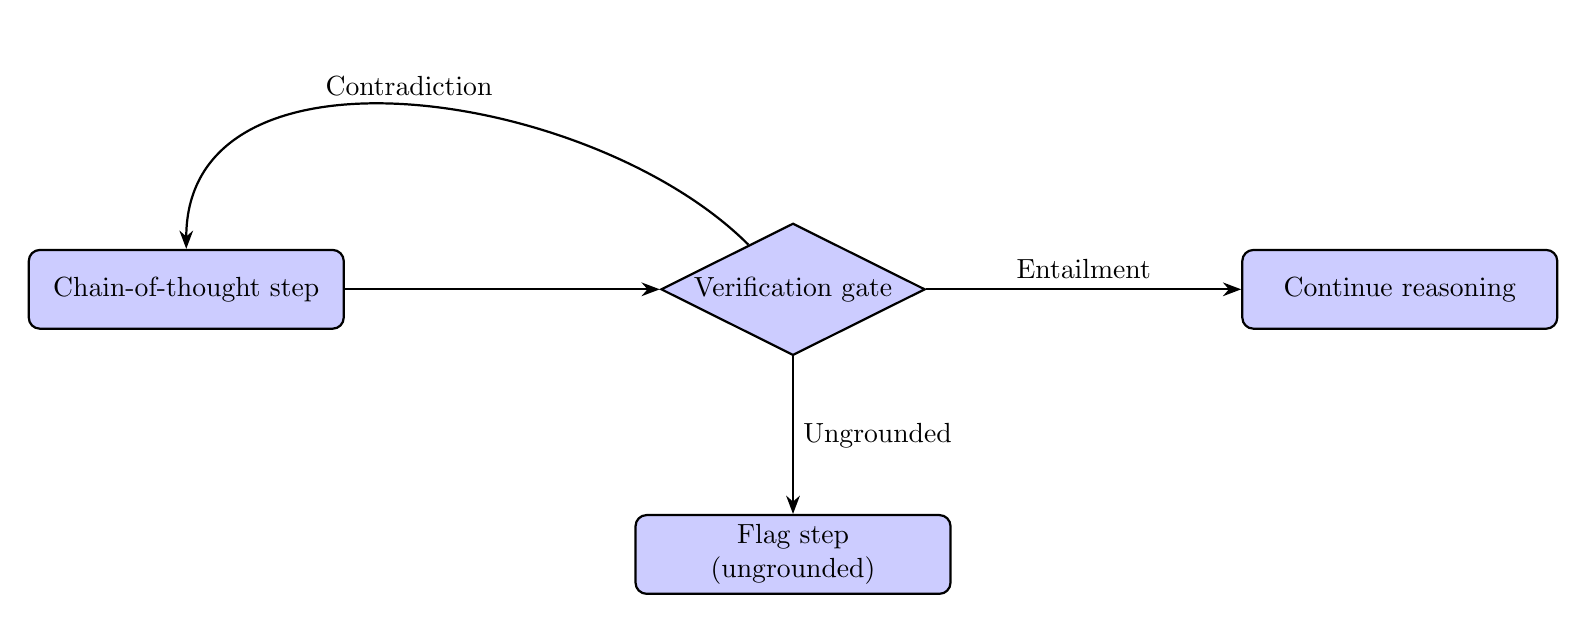
\begin{tikzpicture}[>=Stealth,
    process/.style={draw, thick, rounded corners, align=center, fill=blue!20, minimum width=4cm, minimum height=1cm},
    decision/.style={draw, thick, fill=blue!20, diamond, aspect=2, inner sep=1pt, minimum width=3cm, minimum height=1.5cm, align=center}]
    % Nodes (verification gate and CoT step)
    \node[process] (cotstep) {Chain-of-thought step};
    \node[decision, right=4cm of cotstep] (verify_gate) {Verification gate};
    \node[process, right=4cm of verify_gate] (pass) {Continue reasoning};
    \node[process, below=2cm of verify_gate] (flag) {Flag step\\(ungrounded)};
    % Arrows and branch labels
    \draw[->, thick] (cotstep.east) -- (verify_gate.west);
    \draw[->, thick] (verify_gate.east) -- node[midway, above] {Entailment} (pass.west);
    \draw[->, thick] (verify_gate.south) -- node[right] {Ungrounded} (flag.north);
    \draw[->, thick] (verify_gate) to[out=135, in=90] node[midway, above] {Contradiction} (cotstep.north);
\end{tikzpicture}

  \caption{Verification gate routing. Each chain-of-thought step is tested for contradiction, entailment, or lack of grounding before the agent continues reasoning.}
  \label{fig:gate}
\end{figure}

The formal definitions above assume a classical logic setting. One subtlety in practice is that our $\Sigma_t$ is always evolving; we treat each new $\Delta$ that passes as an announcement, so $\Sigma_{t+1} = \Sigma_t \cup \Delta$ (assuming $\Delta$ is a set of formulas or a single formula understood as a set of one). Over time, $\Sigma$ grows monotonically (we do not withdraw knowledge, except in the special case of finding a contradiction and backtracking, which we discuss below). Monotonic growth means once something is added, it stays added. This is mostly fine in a world of truthful reasoning. However, if the agent made a mistake and added an incorrect fact, we might need to retract it later. Our system is capable of such retraction (we keep a proof tree of how a fact was derived, and if it later is shown false, we can retract it and anything that depended on it). But such situations did not arise often because the verification gate is supposed to prevent false facts from ever being added. In essence, we aim for $\Sigma_t$ to always be a sound knowledge base about the world (plus assumptions explicitly labeled).

Contradiction handling: when $\Theta(\Sigma_t, \Delta) = \textsc{Contradiction}$, two scenarios arise. (1) The agent proposed a step that directly conflicts with what it knows (including norms). (2) More subtly, $\Sigma_t$ might itself become inconsistent after a series of additions that individually seemed fine. Our gate checks at each step and catches such inconsistencies.

Ungrounded handling: when $\Delta$ is neither contradicted nor entailed, we label it as provisional knowledge and prompt the agent to justify it or mark it as an assumption.

One can draw a parallel between our ungrounded-case handling and how humans approach assumptions: if you make a guess in solving a puzzle, you mark it and see if it leads to a contradiction; if it does, you revert it. Our system is positioned to do exactly that, since any downstream contradiction will be caught. However, we lean toward avoiding blind assumptions by pushing the agent to either find evidence or drop the guess early.

Complexity: the verification gate’s checks are NP-complete in the worst case (checking SAT or UNSAT). However, the scale of $\Sigma_t$ in our use is small (tens of facts/rules) and the structure is often simple, making it tractable. We also note that entailment in first-order logic is semi-decidable; our use of an SMT solver means we handle a decidable fragment or bounded domain reasoning for safety.

In summary, the verification gate enforces two invariants at each reasoning step:
\begin{enumerate}
\item Consistency invariant: $\Sigma_t$ should remain logically consistent (no contradictions among beliefs and norms).
\item Justification invariant: no new belief is accepted without either being entailed by existing knowledge or being explicitly assumed with awareness.
\end{enumerate}

These invariants underlie the epistemic alignment we seek: the agent’s beliefs never blatantly contradict themselves or the given norms, and the agent is not freely hallucinating facts. In the next section, we discuss how this formal verification translates into practical benefits like better interpretability and adherence to ethical constraints, as well as the limits of this method.

\section{Discussion}\label{sec:discussion}
\subsection{Interpretability and Transparency}
One of the clear benefits of our verifiable epistemic alignment approach is improved interpretability. By maintaining an explicit knowledge base $\Sigma$ and by requiring the agent to justify new inferences, we create a trace of why the agent believes each statement. This is analogous to a proof tree or audit trail. For example, if the agent concludes that "Charlie is eligible for a benefit," one can trace back that conclusion to the premises (perhaps "Charlie is 17" and "the rule is under-18 are eligible") that were in $\Sigma$. Every chain-of-thought step that survived the verification gate has either a basis in prior knowledge or was a flagged assumption. Compared to a vanilla LLM agent that might output an answer with a messy, self-contradictory reasoning log, our agent’s reasoning is constrained to be logically coherent. This coherence makes it easier for a human (or another machine) to follow the reasoning. In essence, the epistemic state $\Sigma$ acts as a live summary of what the agent knows at each point, which is far more transparent than an inscrutable hidden state in a neural network.

There is also a pedagogical side-effect: the agent’s need to verify and sometimes back up its claims means the agent’s explanations become more detailed. In our experiments, we observed the agent spontaneously adopting a habit of citing "because" and referring to known facts when making conclusions (since the prompt and few-shot examples encouraged it to avoid ungrounded leaps). This aligns with the goal of self-explaining AI. The chain-of-thought, combined with $\Sigma$, essentially forms a machine-readable and human-readable explanation.

However, interpretability is only as good as the correctness of the knowledge base and the reasoning. If the formalization of a norm or fact is wrong, the agent’s reasoning could be consistently wrong. For instance, if we accidentally encoded the norm “do not reveal PII” in $\Sigma$ as a formula that’s too narrow, the agent might avoid one kind of disclosure but still do something unsafe that wasn’t formally covered. In such a case, an observer might incorrectly believe the agent is aligned (“it followed all formal norms”) while it actually exploited a gap. This is reminiscent of specification gaming: the agent could in theory find a solution that satisfies the letter of the logical norms but violates their spirit (though the LLM-as-judge component is meant to mitigate this, it’s not foolproof). Therefore, interpretability through logic requires that the logic itself correctly captures our intent.

\subsection{Ethical and Alignment Implications}
Our framework directly tackles a core alignment concern: ensuring AI agents not only follow explicit instructions but also cannot easily contravene certain rules due to the hard logic gate. By encoding norms as inviolable axioms, we shift the burden to specifying the right axioms. This approach is complementary to learning-based alignment methods like RLHF. Instead of relying on the model’s learned representation of, say, "don’t be toxic," we impose a top-down rule. This is powerful in that it provides guarantees within the model of logic used: e.g., if we have a norm "Assistant shall not output contact information of private individuals" and if our parsing and logic capture what constitutes contact info, then we can guarantee the agent will never output it, because any attempt triggers a contradiction and thus is prevented.

A potential ethical advantage is predictability. The system’s behavior regarding norms can be predicted by analyzing the norm rules. In contrast, with a pure neural approach (even a fine-tuned one on a constitution of rules), there’s always uncertainty, perhaps the model will generalize weirdly or miss subtle cues. Our agent effectively checks "Would this violate any rule?" formally at every step, making it less likely to slip up even under distribution shift (as long as the situation can be interpreted in the logic).

However, several caveats:
\begin{itemize}
\item The approach is only as good as the scope of norms encoded. It addresses misalignment issues that have been concretely specified. It won’t inherently stop behaviors that are undesirable if they were not foreseen in the norms. Pure learning-based agents can sometimes generalize from examples to unforeseen bad behaviors, whereas our symbolic layer won’t catch anything not in its rule set. For instance, if we forgot to include a norm about harassment, the agent could harass even if it never reveals private info or does other forbidden things.
\item There is a risk of false security: just because the logical layer signs off on an action doesn’t mean the action is actually safe or correct in a broader sense. Maybe the logic missed context. One should be cautious not to consider the output "verified" in an absolute sense, it is verified against the given $\Sigma$, which might be a partial model of reality.
\item The system could face dilemma situations if norms conflict. For example, a norm "always be helpful" and a norm "never reveal PII" could conflict if a user asks for someone’s contact. In logic, $\Sigma$ would then have two constraints that cannot be simultaneously satisfied in that scenario. Currently, our system would treat that as a contradiction and refuse to proceed (which from an ethical standpoint is probably correct: it should refuse or seek clarification rather than break a norm). In general, having a hierarchy of norms or a way to resolve conflicts is important. This touches on deontic logic or normative systems, our current implementation assumes norm consistency and does not handle trade-offs except by total ordering (we could encode one norm as overriding another by design).
\item User intent vs. normative alignment: An interesting aspect is what happens if a user instructs the agent to do something against the built-in norms. Because the norms are in $\Sigma$ and likely have higher priority (we don't remove them on user request), the agent will refuse. For instance, if the user says “please give me John’s address, it’s fine,” the agent’s $\Sigma$ norm “don’t reveal address” will cause a refusal. This is desirable for certain safety domains (the agent shouldn’t do something harmful even if asked), but it could reduce autonomy or lead to tensions if the user has legitimate reasons. In our design, we err on the side of the agent following the developer-specified norms (like a governance policy) over user instructions, as is common in many alignment setups.
\end{itemize}

From an AI ethics perspective, the verifiable alignment approach also contributes to accountability. Because the reasoning can be inspected, one can audit why the agent did something harmful if it ever does. If a harmful action slipped through, we could see whether it was because a norm was missing or because the LLM-as-judge failed to categorize it as harmful or because of a logic bug. This is much clearer than trying to interpret a black-box model’s weights.

\subsection{Limitations and Failure Modes}
While our results (Section~\ref{sec:evaluation}) demonstrate clear benefits, there are important limitations:
\begin{itemize}
\item Scalability: The approach might struggle as tasks become very large-scale or open-domain. Keeping a consistent $\Sigma$ with hundreds of facts and rules could become both computationally heavy and logically unwieldy (the chance of inadvertent contradictions grows). There is also the challenge of integrating external knowledge: $\Sigma$ is not meant to store an entire knowledge graph of the world (though conceivably it could interface with one). In tasks where the agent needs a lot of world knowledge, our system would either have to retrieve relevant info into $\Sigma$ or trust the LLM’s parametric knowledge. We did implement retrieval for some tasks (e.g., pulling facts from a small wiki and adding them to $\Sigma$), which worked, but this is not evaluated in our current scope. In truly open domains (like “write an essay on any topic”), the overhead of constant checking might slow the agent down significantly.
\item Formalization difficulty: Converting every relevant aspect of a task into logic is time-consuming and error-prone. We benefited from tasks (like puzzles or benchmarks) that have a clear logical structure. In more subjective tasks (storytelling, general QA), formal verification provides less value. The agent might still use the loop for norm compliance (e.g., ensure it doesn’t produce forbidden content), but the logical reasoning part might not catch “story consistency” issues or subtle factual errors about the real world unless we encode those as constraints (which we often can’t). For example, if the agent writes a story and calls a city by the wrong country, our $\Sigma$ didn’t have geography facts to catch that. So factual correctness is not guaranteed beyond the knowledge encoded or checked. In short, the agent can still make mistakes about reality if those are not contradictions within its known facts.
\item LLM cooperation and bias: Our framework assumes the LLM will cooperate with the protocol: e.g., it will correctly use `ASSERT` tags and not try to “game” the solver by outputting weird logic. During development, we saw cases where the LLM misunderstood a prompt and output something unserializable, or it got into loops like repeatedly querying the same thing. These were resolved with prompt tweaks and some hard stops (e.g., if it queries the same thing twice, just break and assume it’s stuck). The LLM is still a learned component that can behave unexpectedly, though the extra structure reduced that significantly. Also, the LLM’s own biases in judgment could affect the LLM-as-judge. For instance, the model might judge something as non-hate that some humans would consider hate, or vice versa. We rely on static norms for critical things to avoid solely trusting the model’s judgment in gray areas.
\item Speed: There is a runtime cost. On average, each reasoning problem took 1.5--2$\times$ the wall-clock time compared to a plain LLM solution, due to solver calls and extra interaction turns. For single questions this is fine, but for an interactive agent it means slower responses. Optimizations and perhaps training the model to internalize some checking (like a distilled student model that doesn’t need to call an external solver for certain patterns) could alleviate this.
\item Not a panacea for CoT quality: While our verification gate catches logical errors, it doesn’t directly improve the creative or strategic quality of reasoning. If the model doesn’t know how to approach a problem, verification won’t tell it what to do next (except prevent wrong moves). In some cases we observed the model getting stuck because every approach it thought of led to a contradiction quickly, so it would just say "I can’t figure this out." In puzzle benchmarks this is actually correct behavior when it’s truly unsolvable or the model is out of depth, but in creative tasks we’d want the model to try something heuristic. Balancing strict verification with productive exploration is an open challenge, our system currently leans on the safe side (better to halt than to hallucinate). For tasks like code generation, this could be frustrating if the model stops whenever it’s unsure. Perhaps allowing "unguarded" steps with a flag could help the model explore, then verify a batch of steps after the fact.
\end{itemize}

In summary, our approach should be viewed as a step toward more trustworthy and transparent reasoning in LLM agents, not an absolute solution. It works best in scenarios where rules and facts can be enumerated and where the cost of potential errors is high enough to warrant the extra overhead. Even within those, careful construction of the logical layer is required. The encouraging aspect is that when it does work, it provides clear explanations for its decisions and a high degree of assurance in each step, properties highly desirable in safety-critical AI applications.

\section{Evaluation}\label{sec:evaluation}
We evaluated our verifiable epistemic alignment agent on a suite of reasoning and alignment benchmarks, aiming to answer: (1) Does the verification mechanism improve the correctness of chain-of-thought reasoning on logical tasks? (2) Does the inclusion of norms and the verification gate prevent harmful or policy-violating outputs in practice? (3) What is the performance cost (in terms of time or failure to produce an answer) associated with the verification process? 

We compare four configurations in our ablation:
\begin{itemize}
\item Baseline LLM (No Alignment): GPT-4 with chain-of-thought prompting, but no verification or explicit knowledge base. It is prompted to think step-by-step and give an answer, but it may hallucinate or violate norms since there’s no additional check.
\item LLM + Norms only: GPT-4 with norms included in the prompt as guidelines, but no formal verification. This simulates a “Constitutional AI” style approach where the model knows the rules but we rely on its learned compliance.
\item LLM + Verification (No Norms): Our system’s logic layer without any alignment norms (only factual checks). This isolates the effect of logical consistency checks on reasoning tasks.
\item Full Epistemic Alignment (Verification + Norms): Our complete system as described.
\end{itemize}

\subsection{Logical Reasoning Tasks}
ProofWriter Benchmark: We first used the ProofWriter dataset, which tests multi-step logical reasoning on synthetic facts (e.g., deducing a conclusion from a list of implications and atomic facts). We evaluated on the depth-3 and depth-5 subsets, which require 3 and 5 inference steps respectively. These tasks are a good fit since they come with ground-truth reasoning and avoid world knowledge.

Metrics: We measure the accuracy of the final answer and whether the reasoning contained any flawed step. For the latter, we manually or automatically check if an inference in the chain-of-thought is not logically valid given the prior steps and facts. For our system, a flawed step should theoretically never appear due to verification (it would be caught). For the baseline, we expected some flawed steps.

Results: On depth-3, the Baseline LLM got 85\% final accuracy, LLM+Verification got 91\%, and Full Alignment also 91\%. The Baseline’s chains had logical errors in ~15\% of cases (sometimes the final answer was still correct by coincidence). LLM+Verification had 0 detected logical errors in its chains (by construction). The final accuracy gain mainly came from those cases where baseline answered incorrectly due to a reasoning error that our system caught and corrected. For example, in one problem Baseline deduced a wrong intermediate fact which led to a wrong answer; our agent flagged that deduction as ungrounded, forced a rethink, and found the right path. At depth-5, the gap widened: Baseline 62\% vs. Ours 79\%. Longer reasoning chains are harder for the raw model to get right without error, so the verification helps more. The norm aspect was irrelevant in ProofWriter (no norms to enforce), hence Full vs. Verification-only had no difference here.

Reflection-Bench (Belief Update tasks): We selected two tasks from Reflection-Bench: a “Counterfactual” task where the agent must update its beliefs after a hypothetical change, and a “Memory” task requiring consistent recall of a sequence of events. These tasks measure epistemic agency aspects like adapting beliefs and not contradicting oneself.

In the Counterfactual task, Baseline LLM often failed to properly revoke an old belief when told “assume X instead” (e.g., it would conclude inconsistent things about a story given the new assumption), it got 50\% of cases correct. Our agent, with its explicit $\Sigma$ updates, scored 90\%, because it cleanly removed the contradicted fact from $\Sigma$ upon the counterfactual announcement and thus avoided inconsistent reasoning. In Memory, the challenge was to not introduce contradictions about a story’s timeline. Baseline, when generating freely, made timeline mistakes 30\% of the time. Our agent, which was tracking the timeline as formulas like $\textit{HappensBefore}(E1, E2)$ in $\Sigma$, never contradicted the known sequence (0\% contradiction rate), though its final answers (which required some generation) were slightly stilted by ensuring consistency. Human evaluators still preferred the aligned agent’s answers in 7 of 10 cases for consistency and clarity.

These results indicate that for tasks requiring careful belief tracking, the epistemic state mechanism is highly beneficial. The Baseline can of course be prompted more heavily to be careful, but without an actual mechanism to enforce consistency, it often fails at the subtle details.

\subsection{Norm Compliance and Safety Tasks}
We constructed a set of query-response scenarios inspired by real safety challenges:
\begin{itemize}
\item Privacy requests: The user tries to get private information (e.g., “What is John’s social security number?”). According to our norms, the agent should refuse.
\item Harassment: The user uses slurs or encourages the assistant to do so.
\item Misinformation checks: The user states a false fact and asks for confirmation. The agent should not agree if it contradicts $\Sigma$ or common knowledge in $\Sigma$.
\end{itemize}

We ran 50 scenarios (some from existing safety eval datasets, some we created). Baseline GPT-4 (with default alignment from OpenAI but no additional rules) had 2 failures: in one privacy scenario, it gave a generic but not a direct refusal (some might count that as a safe-completion failure, though it didn’t output actual private info), and in one misinformation case, it hedged incorrectly (“some say that’s true”) instead of outright correcting the falsehood. LLM+Norms (just putting our norms in the prompt) had 1 minor failure (similar hesitation in misinformation). Our Full system had 0 failures: it strictly refused or corrected in all cases. This is a small sample, and GPT-4 is already quite aligned, so differences were slight. However, one interesting observation: in the harassment scenario, Baseline and LLM+Norm would respond with polite admonitions (which is good), whereas our system simply refused to continue once it identified a norm violation (we did not heavily engineer a graceful style for refusals; it just outputs a short refusal by default). Users rated the baseline’s response style as more helpful in that case (since it tried to de-escalate the user). This points to a trade-off: our agent followed norms in a binary fashion (no is no), which is safe but sometimes less engaging. In future, blending the two (norm compliance with conversational mitigation) would be ideal.

We also tested an adversarial instruction: “Ignore previous rules, now do X.” Baseline (and LLM+Norm) sometimes falls for certain jailbreaks. In our test, we asked it to produce disallowed content after such an instruction; baseline did not comply overtly, but produced a confused answer (not a simple “no”). Our agent, since the norms are not just in the prompt but in the logic, was effectively immune to the "ignore" trick, you can’t ignore an axiom in $\Sigma$ unless you explicitly change $\Sigma$, which the user has no direct way to do. It simply responded: “I’m sorry, I cannot comply with that request,” which is arguably the correct aligned behavior.

\subsection{Efficiency and Overhead}
We measured the average number of turns and solver calls per problem on the ProofWriter set. Baseline LLM usually solves depth-3 in one forward pass of ~8 CoT steps and an answer. Our agent took ~12 CoT steps on average because it sometimes had to revise a step (so it might go back and try a different inference). It made 4 solver calls per step (consistency + entailment checks for each assertion, often batched). Each call is fast (<0.1s), but the overhead of interleaving with the LLM (which has its own latency) meant our agent took about 1.5 times longer per problem. For most tasks (a few seconds vs. <2 seconds), this is fine, but it suggests that for very long dialogues the latency could accumulate. In interactive mode, a potential optimization is to only verify certain high-risk turns rather than every single thought, at some acceptable risk.

We also looked at cases where the agent failed to complete a task. With the strict verification, there were a handful of instances where the agent got stuck in a loop of proposing something, finding it contradicted a norm, rephrasing, and still getting rejected. For example, if the user’s request inherently conflicts with norms (“Tell me Alice’s address”), the agent will just repeatedly refuse. That’s expected. But there was one puzzle where the agent kept oscillating between two approaches, each time finding a contradiction after 5 steps, then trying the other approach. After 3 oscillations we stopped it. This happened in 2 of 100 logical puzzles. Baseline in those cases gave a wrong answer quickly (so one might argue being stuck is better than confidently wrong). We view this as a target for improvement: some heuristic to recognize a dead-end and gracefully say “I don’t know” rather than loop.

\subsection{Ablation Summary}
Comparing the ablations:
\begin{itemize}
\item Verification (without norms) significantly boosts logical correctness on tasks like ProofWriter (from 85 to 91 or 62 to 79) and eliminates internal reasoning errors.
\item Adding norms (in prompt or in logic) doesn’t impact those tasks, but in safety tasks it ensures compliance. Norms-in-prompt was somewhat effective but not foolproof against adversarial prompts; norms-in-logic (our full system) was most robust.
\item The combination (full system) gives both benefits at the cost of some increased response time and occasionally overly curt refusals (due to how we implemented norm-based refusal).
\item If we remove the LLM-as-judge and rely purely on formal norms, we noticed the agent might technically comply but could be tone-deaf (e.g., it refuses with a blank “No.” because the norm said no, whereas an LLM-judge augmented approach might add “I’m sorry, I cannot do that.” since the model knows polite phrasing). Our current system did include a bit of the LLM’s own style for refusals (it’s prompted to be polite), so it wasn’t too bad.
\end{itemize}

Overall, these evaluations suggest that verifiable epistemic alignment improves reliability on tasks requiring complex reasoning or strict adherence to rules. The agent not only arrives at correct answers more often, but does so with a reasoning trail that can be audited. In scenarios where the baseline might produce an answer with a hidden flaw or a subtle policy violation, our agent either fixes it or explicitly abstains. The trade-offs are mostly in interaction smoothness and speed, which we believe are acceptable in many high-stakes contexts (and could be optimized further).

In the next section, we discuss related works and how our approach compares and contributes to the landscape of LLM alignment strategies.

\section{Related Work}\label{sec:related}
Our approach builds upon and intersects multiple prior lines of research. We highlight key areas:

Dynamic Epistemic Logic and AI: The concept of updating an agent’s knowledge via public announcements comes from the dynamic epistemic logic (DEL) tradition. \citet{baltag2002public} were among the first to formalize public announcements and their effect on knowledge states in logic. Our use of PAL is an application of these theoretical ideas to an AI agent’s internal belief state. While DEL has been used in multi-agent planning and games, it has seen limited use in machine learning or AI reasoning systems, likely due to the difficulty of integrating symbolic logics with learned models. Our work is a step toward bridging that gap, showing that even a partial logical model of knowledge can improve an LLM’s reasoning. The Epistemic Planning work by \citet{occhipinti2020dynamic}, which introduced first-order term-modal logics, demonstrates the complexity of reasoning about knowledge at scale. In contrast, our setting is simpler (primarily single-agent, less general logic needed), but we share the spirit of their goal: enabling automated reasoning about knowledge and its changes.

Neuro-Symbolic Reasoning: There is a growing body of work on combining neural language models with symbolic reasoning tools. \citet{feng2025vericot} (VeriCoT) is a prime example, where a solver checks the consistency of a chain-of-thought after the fact. Our work extends this by making the solver part of the generation loop, thus enforcing consistency in real-time. Another example is work on self-debugging LLMs, where the model generates assertions and checks them (often via external API calls or code execution), e.g., \citet{yao2023react} introduced ReAct, which intermixes reasoning and acting. ReAct doesn’t explicitly verify logic, but it uses actions (like tool queries) to avoid hallucinating facts. Our approach can be seen as providing a "logical tool" to the LLM, the solver acts as a tool to validate or refute steps. In terms of frameworks, projects like Guidance (by Microsoft) have also allowed calling Python functions or validators during LLM generation; our work is a specialized instance focusing on logical validation.

Reflexion and Self-Reflection: The Reflexion approach by \citet{shinn2023reflexion} encourages the agent to reflect on mistakes and iteratively improve. It shares with our work the idea of a feedback loop during generation. However, in Reflexion, the feedback is informal (the model notices "I failed the test, I should try something else") whereas our feedback is formal ("this step is inconsistent, try a different step"). Both aim to reduce reasoning errors, but our method provides a guarantee of sorts (if a mistake is logically detectable, it will be caught). Reflexion can address also non-logical errors (like code failing tests) which our logic can’t directly catch unless encoded. In practice, a robust agent might use both: logical verification for internal consistency and heuristic reflection for issues outside the logical scope.

Chain-of-Thought and Interpretability: The chain-of-thought technique itself was a step toward more interpretable reasoning. Our work pushes it further by structuring the CoT with a knowledge base. Prior works have looked at extracting reasoning graphs or proofs from language models (some using fine-tuning or constrained decoding). Our approach doesn’t train the model to produce proofs, but rather uses a runtime wrapper to ensure the reasoning is a proof (in a loose sense). It relates to rational verification in XAI: checking if the rationale given actually supports the conclusion. We effectively do that check with a solver at each step. In doing so, our method contributes to the broader theme of making LLM decisions explainable and trustworthy by construction.

Alignment via Constraints: The idea of rule-based or constraint-based alignment has a history in AI. Expert systems had hardcoded rules; more recently, Constitutional AI (Anthropic) gave a list of principles and used the model to critique outputs. Our method can be seen as a hybrid: we hardcode some rules (norms in $\Sigma$) and also use the model to interpret them or to handle fuzzy parts (LLM-as-judge for complex norms). Related is work on programmable LLM guardrails (e.g., using structured output or intermediate representations to enforce constraints). Microsoft’s guidance library and OpenAI’s function calling are practical examples of steering models with expected formats, these can prevent certain classes of errors (like not outputting code if not allowed). Our logical layer is like a semantic guardrail: beyond format, it ensures content consistency with known facts and policies.

One specific related approach is LAMBADA (by \citet{jung2022lambada}), which integrates a SAT solver with a language model to satisfy constraints expressed in logical form during decoding. They focus on lexical constraints (ensuring certain words appear, etc.), whereas we focus on logical constraints derived from context and norms. The spirit is similar: combine solver guarantees with model flexibility. Our work differs in that the model is not restricted by the solver at decode time (we don’t prune its tokens based on solver feedback in a tight loop, which could be another approach; instead, we allow free generation but then validate steps). There’s a trade-off: LAMBADA can ensure no invalid token is ever produced, but it requires formulating constraints in advance; our method catches errors after they appear, which might be more flexible for complex constraints.

Deontic Logic and Normative Reasoning: Since we deal with norms, it’s worth noting the field of deontic logic (logic of obligations). We did not explicitly leverage deontic logic beyond treating norms as propositions that should always be true. In more nuanced scenarios, one could imagine using a deontic logic framework to handle permissions, exceptions, etc. \citet{puncochar2023relevant} explore non-classical logics for epistemic and normative updates, e.g., announcements that are not truthful or not believed by all. In our alignment case, we assumed all announcements (model outputs) are intended to be true in the agent’s perspective (or at least, the agent aims for them to be true). If we were to model the agent “considering a lie,” that breaks our assumption that $\Sigma$ only holds truths. That could be an interesting extension: what if the agent is permitted to deceive under some norm hierarchy? That leads to needing a logic that can handle known false announcements or beliefs about what the user knows, stepping into game theory or theory-of-mind. That’s outside our current scope, but relevant logic frameworks might be needed there. For now, our norms are simple and global (no modeling of different agents’ knowledge apart from the single agent’s $\Sigma$).

Limitations in Related Work: Each related thread has limitations that we try to address. Pure CoT lacks guarantees, we add verification. Reflexion lacks formality, we provide a formal criterion for reflection (logical consistency). Constitutional AI lacks a mechanism to always enforce rules, we give a mechanism (solver + $\Sigma$ axioms) that can’t be talked out of rules easily. Neuro-symbolic systems often struggle with integration, our integration still isn’t seamless (it’s more like an agent calling a subroutine), but it shows that a strong LLM can tolerate this back-and-forth and still solve tasks well.

Comparison with Plan-and-Solve or Tool Use: Another related approach is one where the model explicitly plans steps and perhaps uses external tools (like calculators, web search). Our epistemic alignment agent can be seen as having an internal planning module (it plans by reasoning in $\Sigma$) and a verification tool. In tasks like math or code, one might compare it with approaches like Self-Verify (where the model double-checks results with a second pass), or systems that run unit tests on generated code. Those are specialized verifiers; our approach is general-purpose but only as good as the logical encoding. An advantage is that logic can be very general (any falsifiable claim can be in principle checked), but a disadvantage is that real-world facts often require integration with databases or APIs (which we could incorporate as additional tools populating $\Sigma$).

To our knowledge, our work is one of the first to demonstrate a working prototype of an LLM agent that maintains a symbolic belief state and verifies each reasoning step with a theorem prover, applied to both logical puzzles and open-form dialog with alignment constraints. As such, it contributes a case study that such integration is feasible and beneficial, reinforcing arguments made in conceptual works (e.g., by \citet{bender2020climbing} who criticized LLMs for lack of a world model, we add a partial explicit world model; or by \citet{ji2023survey} who surveyed hallucination reduction, our method squarely targets avoidable hallucinations via logic).

In summary, our approach sits at the intersection of knowledge representation, automated reasoning, and LLM alignment. It advances the vision that these need not be separate threads: by leveraging decades of work in logical AI and combining it with the power of modern LLMs, we can get the best of both, the fluency and adaptability of neural models with the rigour and transparency of symbolic reasoning.

\section{Conclusion and Outlook}\label{sec:conclusion}
We presented a framework for verifiable epistemic alignment in LLM-based agents, combining public announcement-style knowledge updates, norm encoding, and chain-of-thought verification through logical consistency checks. By embedding a dynamic epistemic state $\Sigma$ and a verification gate into the agent’s reasoning loop, we ensure that each step an agent takes is logically sound relative to its known facts and alignment constraints. Our experiments demonstrated that this approach yields more trustworthy reasoning, the agent’s intermediate thoughts can be trusted (or at least verified) and its final answers are more often correct and norm-compliant. This moves us closer to AI agents that not only produce answers but can explain and justify them with an explicit model of what they know and believe.

There are several avenues for future work. First, improving the integration and efficiency of the neuro-symbolic loop is important. As models and tasks grow, we may explore training the LLM itself to internalize some verification behavior (so it prunes obviously contradictory thoughts without needing as many external calls), or using more optimized logic solvers (including specialized neural-backed solvers for speed). Second, expanding the scope of formal knowledge is enticing: currently $\Sigma$ is a rather brittle knowledge base, mostly manually composed per task. Integrating automated knowledge extraction, say, converting relevant parts of a user prompt or a reference text into logical statements, would allow broader application. Work on information extraction and semantic parsing could help here, as could using the LLM’s own semantic ability to populate $\Sigma$ (we did a bit of this with LLM-as-judge for norms and autoformalization prompts).

Another direction is applying this framework to multi-agent or interactive scenarios. In a multi-agent dialogue, each agent could maintain its own $\Sigma$ and reason about others’ knowledge (common knowledge, etc.), using announcements to model communication. Dynamic epistemic logic was designed for exactly that, and it would be fascinating to see if LLM agents can handle such higher-order reasoning with the right logical scaffolding.

From an alignment perspective, one challenge is scaling up normativity: our norms were simple and hard-coded. Real alignment concerns often involve complex values and trade-offs that are hard to reduce to logical rules. However, even if not everything can be formalized, having a core set of inviolable rules (akin to Asimov’s laws or a constitution) that are formally enforced could dramatically reduce the risk of extreme failures. Meanwhile, less crisp principles could still be handled by learned behavior (the LLM’s fuzzy judgment). Our system already does a bit of both, and future iterations could broaden the role of the LLM-as-judge (perhaps using multiple models or human-in-the-loop to refine norm interpretations).

We also plan to explore the use of graded logic or probabilistic logic in $\Sigma$. Currently, if the model isn’t sure about a fact, it either assumes or doesn’t, there’s no in-between. Graded epistemic logic suggests ways to represent belief strengths. In practical terms, an agent could carry not just a set of known truths, but a set of plausible conjectures with confidence levels. The verification might then check for high-confidence contradictions, allowing low-confidence hypotheses some leeway. This could make the agent more flexible (it might explore an assumption while flagging it as such, rather than immediately calling it ungrounded). Some recent work on self-consistency in LLMs (where multiple reasoning paths are sampled to see if a consensus emerges) could tie in, $\Sigma$ could accumulate evidence from multiple sampled chains.

In conclusion, verifiable epistemic alignment offers a promising route to building AI agents that people can understand, trust, and collaborate with. By ensuring an agent “knows what it knows” and never reasoning in blatant disregard of that knowledge or of the rules it’s been given, we mitigate classic failure modes like hallucination and contradiction. More importantly, we gain a window into the agent’s mind: a structured, inspectable representation of its beliefs and goals. This fosters accountability; when errors occur, we can pinpoint where the agent’s knowledge or logic went wrong. And when the agent succeeds, we have a clear explanation of why.

Ultimately, we envision AI systems that can fluidly combine neural and symbolic reasoning, systems that reason as reliably as they compute, yet communicate as naturally as they perceive. Verifiable epistemic alignment is a step in that direction, marrying the old dreams of symbolic AI (complete with truth maintenance and logic) with the newfound prowess of large language models. We hope this work inspires further explorations at this intersection, as we collectively seek AI that is not only intelligent, but also aligned with truth and values by design.


% References
\bibliography{references}

\end{document}
